%%%%%%%%%%%%%%%%%%%%%%%%%%%%%%%%%%%%%%%%%%%%%%%%%%%%%%%%%%%%%%%%%%%%%%%%%%%%%%
%% Online Supplement -- Signal, Image and Video Processing (Springer Nature)
%%
%% Companion to main.tex.  Single-column deliberately: supplements are read on
%% screen, and the wide tables here do not fit a two-column measure.
%% Build:  pdflatex -> bibtex -> pdflatex -> pdflatex
%%%%%%%%%%%%%%%%%%%%%%%%%%%%%%%%%%%%%%%%%%%%%%%%%%%%%%%%%%%%%%%%%%%%%%%%%%%%%%

\documentclass[pdflatex,sn-basic,Numbered]{sn-jnl}

\usepackage{graphicx}
\usepackage{amsmath,amssymb,amsfonts}
\usepackage{booktabs}

% Supplement numbering: S1, S2, ... for sections, tables, figures and equations.
\renewcommand{\thesection}{S\arabic{section}}
\renewcommand{\thetable}{S\arabic{table}}
\renewcommand{\thefigure}{S\arabic{figure}}
\renewcommand{\theequation}{S\arabic{equation}}

\raggedbottom

\begin{document}

\title[Online Supplement]{Online Supplement to ``Confinement-loss prediction in
photonic crystal fiber SPR sensors: kernel surrogates versus generative data
augmentation''}

\author*[1]{\fnm{Mohammad Khaleel} \sur{Hammoud}}\email{mhmdkhalil.h@gmail.com}

\author[1]{\fnm{Cem} \sur{Kalyoncu}}\email{ckalyoncu@eul.edu.tr}

\author[1]{\fnm{Ahmet} \sur{Yasli}}\email{ayasli@eul.edu.tr}

\affil*[1]{\orgdiv{Department of Computer Engineering}, \orgname{European
University of Lefke}, \orgaddress{\city{Lefke}, \country{Northern Cyprus, TR-10
Mersin, Turkey}}}

\abstract{This supplement contains material supporting the main article that is
not required to follow its argument: the dual formulation of support vector
regression and its optimality conditions (Sect.~\ref{sup:svr}), the Bayesian
hyperparameter search space and its outcome (Sect.~\ref{sup:bayes}), per-fold
leave-one-geometry-out results (Sect.~\ref{sup:logo}), the generative model
configuration and the contradiction-search protocol (Sect.~\ref{sup:gan}), a
Gaussian process kernel and regulariser ablation (Sect.~\ref{sup:gpr}), and the
complete Monte Carlo tolerance tables (Sect.~\ref{sup:mc}). Section, table,
figure and equation numbers are prefixed with S; citations refer to the
reference list of the main article, reproduced here for convenience.}

\keywords{Supplementary material}

\maketitle

%%%%%%%%%%%%%%%%%%%%%%%%%%%%%%%%%%%%%%%%%%%%%%%%%%%%%%%%%%%%%%%%%%%%%%%%%%%%%%
\section{Support vector regression: dual formulation}\label{sup:svr}

The main article states the primal problem, Eqs.~(3)--(4). The derivation below
is the standard one~\cite{smola2004}, reproduced here so that the argument of
Sect.~5.2 of the main article can be followed without a second source.
Introducing Lagrange multipliers $\alpha_i, \alpha_i^{*} \ge 0$ for the two
$\epsilon$-tube constraints and $\eta_i, \eta_i^{*} \ge 0$ for the
non-negativity of the slacks gives the Lagrangian

\begin{align}
L = {}& \frac{1}{2}\|w\|^{2} + C\sum_{i=1}^{n}(\xi_i + \xi_i^{*})
      - \sum_{i=1}^{n}(\eta_i\xi_i + \eta_i^{*}\xi_i^{*}) \nonumber\\
  & - \sum_{i=1}^{n}\alpha_i\!\left(\epsilon + \xi_i - y_i
      + \langle w, x_i\rangle + b\right) \nonumber\\
  & - \sum_{i=1}^{n}\alpha_i^{*}\!\left(\epsilon + \xi_i^{*} + y_i
      - \langle w, x_i\rangle - b\right).
\label{eq:lagrangian}
\end{align}

Setting the partial derivatives with respect to the primal variables to zero
yields the saddle-point conditions

\begin{equation}
w = \sum_{i=1}^{n}(\alpha_i - \alpha_i^{*})x_i, \qquad
\sum_{i=1}^{n}(\alpha_i - \alpha_i^{*}) = 0, \qquad
\alpha_i^{(*)} + \eta_i^{(*)} = C,
\label{eq:saddle}
\end{equation}

and substituting them back removes the primal variables entirely, leaving the
dual

\begin{align}
\max_{\alpha,\alpha^{*}} \quad
& -\frac{1}{2}\sum_{i,j=1}^{n}(\alpha_i - \alpha_i^{*})(\alpha_j - \alpha_j^{*})
   K(x_i,x_j) \nonumber\\
& - \epsilon\sum_{i=1}^{n}(\alpha_i + \alpha_i^{*})
  + \sum_{i=1}^{n}y_i(\alpha_i - \alpha_i^{*}),
\label{eq:dual}
\end{align}

subject to $\sum_i (\alpha_i - \alpha_i^{*}) = 0$ and
$\alpha_i, \alpha_i^{*} \in [0, C]$. The prediction is then

\begin{equation}
f(x) = \sum_{i=1}^{n}(\alpha_i - \alpha_i^{*})K(x_i, x) + b.
\label{eq:prediction}
\end{equation}

Two properties of \eqref{eq:dual}--\eqref{eq:prediction} matter for the
argument in the main article. First, the inputs enter only through the kernel
$K(x_i,x_j)$, so the RBF map never has to be formed explicitly. Second, the
Karush-Kuhn-Tucker complementarity conditions

\begin{equation}
\alpha_i(\epsilon + \xi_i - y_i + \langle w,x_i\rangle + b) = 0, \qquad
(C - \alpha_i)\xi_i = 0,
\label{eq:kkt}
\end{equation}

force $\alpha_i = \alpha_i^{*} = 0$ for every sample strictly inside the
$\epsilon$-tube. The expansion in \eqref{eq:prediction} is therefore supported
only by samples on or outside the tube boundary. On this dataset that
concentrates the fit near the resonance transition, where the response is
steepest, and it is why the model tolerates a training set of 432 samples.

Condition \eqref{eq:kkt} also explains the contrast with Gaussian process
regression~\cite{rasmussen2006} in Sect.~5.2 of the main article. A pair of near-duplicate inputs
carrying contradictory targets simply saturates at $\alpha_i = C$: both points
become bounded support vectors, the fitted function is worse, but nothing in
\eqref{eq:dual} becomes ill-posed. There is no matrix to invert.

%%%%%%%%%%%%%%%%%%%%%%%%%%%%%%%%%%%%%%%%%%%%%%%%%%%%%%%%%%%%%%%%%%%%%%%%%%%%%%
\section{Bayesian optimisation of the SVR hyperparameters}\label{sup:bayes}

Table~\ref{tab:searchspace} gives the search space and the selected
configuration. The acquisition function is expected improvement over a Gaussian
process surrogate on the hyperparameter space~\cite{snoek2012}, with 32
evaluations. Each
candidate is scored by three-fold cross-validated mean squared error computed on
the training partition only, so no information from the held-out geometry enters
the selection.

\begin{table}[h]
\caption{Hyperparameter search space and the configuration selected by Bayesian
optimisation. Priors are log-uniform because the three parameters span several
orders of magnitude and the objective is far more sensitive to their order than
to their mantissa.}\label{tab:searchspace}
\begin{tabular*}{\textwidth}{@{\extracolsep\fill}llll}
\toprule
Parameter & Range & Prior & Selected \\
\midrule
$C$ (box constraint)  & $[1, 2000]$          & log-uniform & 2000 \\
$\gamma$ (RBF width)  & $[10^{-4}, 1]$       & log-uniform & 0.0172 \\
$\epsilon$ (tube)     & $[10^{-4}, 10^{-1}]$ & log-uniform & $10^{-4}$ \\
Kernel                & RBF (fixed)          & ---         & RBF \\
\midrule
Evaluations           & 32                   & ---         & --- \\
Inner validation      & 3-fold CV            & ---         & --- \\
\botrule
\end{tabular*}
\footnotetext{The selected $C$ and $\epsilon$ sit at their respective range
limits, which indicates the optimum lies at or beyond the boundary: the fit
prefers a hard penalty and an almost vanishing insensitivity tube. Widening the
range is unlikely to change the fit materially -- at $\epsilon = 10^{-4}$ the
tube is already far narrower than the residual scale -- but the boundary
solution should be reported rather than presented as an interior optimum.}
\end{table}

The selected width $\gamma = 0.0172$ is small relative to the unit-cube extent
of the scaled inputs, giving a broad kernel: the model is smoothing over a
substantial fraction of the design space rather than fitting locally, which is
the expected regime when nine geometries must support prediction on a tenth.

%%%%%%%%%%%%%%%%%%%%%%%%%%%%%%%%%%%%%%%%%%%%%%%%%%%%%%%%%%%%%%%%%%%%%%%%%%%%%%
\section{Per-fold leave-one-geometry-out results}\label{sup:logo}

Table~\ref{tab:logo} gives the fold-level results summarised in Table~2 of the
main article, and Fig.~\ref{fig:logo} shows them graphically.

\begin{table}[h]
\caption{Held-out mean squared error for each of the nine geometric
configurations, with and without GAN-generated training samples. Folds run down
the rows; the final two rows give the summary statistics quoted in the main
article.}\label{tab:logo}
\begin{tabular*}{\textwidth}{@{\extracolsep\fill}lccc}
\toprule
Held-out geometry & SVR, real data only & SVR + GAN samples & Ratio \\
\midrule
D1 & 0.128 & 1.074 & 8.41 \\
D2 & 0.379 & 0.848 & 2.24 \\
D3 & 0.257 & 0.321 & 1.25 \\
D4 & 0.212 & 0.261 & 1.23 \\
D5 & 0.829 & 0.487 & 0.59 \\
D6 & 0.121 & 1.359 & 11.27 \\
D7 & 0.131 & 0.684 & 5.21 \\
D8 & 0.096 & 2.200 & 22.83 \\
D9 & 0.060 & 0.194 & 3.24 \\
\midrule
Mean               & 0.246 & 0.825 & --- \\
Standard deviation & 0.226 & 0.610 & --- \\
\botrule
\end{tabular*}
\footnotetext{Ratio is augmented MSE divided by real-only MSE; values above one
indicate augmentation made that fold worse.}
\end{table}

\begin{figure}[h]
\centering
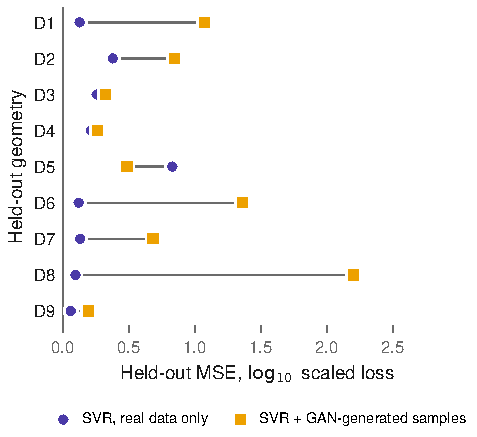
\includegraphics[width=0.60\textwidth]{figs/figS1_logo_folds.pdf}
\caption{Per-fold held-out error with and without GAN augmentation. Each
connector spans one geometry, so the direction of change is read directly. Eight
of the nine folds move to the right, that is, get worse under
augmentation.}\label{fig:logo}
\end{figure}

The per-fold view supports a claim the averages cannot. Augmentation is not a
uniform penalty: it is nearly neutral on D3 and D4, mildly helpful on D5, and
catastrophic on D8, where the error grows by a factor of 23. This is the
signature of synthetic samples that contradict specific regions of the design
space rather than of noise added evenly across it. D5 is the only fold where
augmentation helps, and it is also the fold with the worst real-only error --
consistent with extra samples helping only where the real coverage was
genuinely thin.

%%%%%%%%%%%%%%%%%%%%%%%%%%%%%%%%%%%%%%%%%%%%%%%%%%%%%%%%%%%%%%%%%%%%%%%%%%%%%%
\section{Generative model and contradiction search}\label{sup:gan}

\subsection{WGAN-GP configuration}

The generative model is a Wasserstein GAN with gradient
penalty~\cite{gulrajani2017}, reimplementing the architecture reported by Zelaci
et al.~\cite{zelaci2021} so that the augmentation experiment tests their
procedure and not a variant of it. Table~\ref{tab:wgan} gives the configuration.

\begin{table}[h]
\caption{WGAN-GP configuration used for the augmentation experiments.
Generator and critic are given side by side; the training column applies to
both.}\label{tab:wgan}
\begin{tabular*}{\textwidth}{@{\extracolsep\fill}llll}
\toprule
Property & Generator & Critic & Training \\
\midrule
Hidden layers    & 5                & 5                    & --- \\
Units per layer  & 128              & 32                   & --- \\
Activation       & LeakyReLU (0.2)  & LeakyReLU (0.2)      & --- \\
Normalisation    & none             & batch normalisation  & --- \\
Output width     & 8                & 1                    & --- \\
\midrule
Optimiser        & ---              & ---                  & Adam, $\beta = (0.5, 0.9)$ \\
Learning rate    & ---              & ---                  & $10^{-4}$ \\
Batch size       & ---              & ---                  & 32 \\
Critic steps     & ---              & ---                  & 5 per generator step \\
Epochs           & ---              & ---                  & 2000 \\
\botrule
\end{tabular*}
\end{table}

The generator is trained on the concatenation of the min-max scaled input
features and the min-max scaled target, so it models the joint distribution of
geometry and response. This is the property the contradiction search exploits:
nothing in the objective requires the generated joint samples to be consistent
with a single-valued map from geometry to loss.

\subsection{Contradiction search protocol}

We drew 50,000 samples from the trained generator and, for each, found its
nearest neighbour in the scaled feature space under the Euclidean metric,
excluding the sample itself. For a pair at feature distance $\delta$ with
targets differing by $\Delta y$, we ranked by

\begin{equation}
\rho = \frac{\Delta y}{\max(\delta,\, 10^{-6})},
\label{eq:ratio}
\end{equation}

which measures how steeply the generated response surface must rise to
accommodate the pair. Table~4 of the main article reports the three pairs with
the largest $\rho$. Ranking by $\rho$ rather than by $\delta$ alone is
deliberate: a pair that is merely close is unremarkable, and it is the
combination of proximity and target disagreement that is physically
impossible.

The feature space for this search is the seven-dimensional set the generator was
trained on -- analyte index, real effective index, wavelength, pitch and the
three hole diameters -- min-max scaled to the unit cube. The floor of $10^{-6}$
in \eqref{eq:ratio} guards the division for coincident samples.

Note that $\rho$ is a diagnostic, not an estimator: its absolute magnitude
depends on the scaling of both axes and should not be compared across datasets.
Within this experiment it is the ordering that carries the information.

%%%%%%%%%%%%%%%%%%%%%%%%%%%%%%%%%%%%%%%%%%%%%%%%%%%%%%%%%%%%%%%%%%%%%%%%%%%%%%
\section{Gaussian process kernel and regulariser ablation}\label{sup:gpr}

Section~5.2 of the main article attributes the GPR collapse to
ill-conditioning of $[K + \sigma_n^{2}I]$. If that account is right, the
collapse should depend on how the inversion is regularised. Table~\ref{tab:gpr}
tests this by crossing the two available regularisers -- an additive white-noise
kernel term (WK)~\cite{rasmussen2006} and \texttt{scikit-learn}'s explicit
jitter $\alpha$ -- against real and augmented training data.

\begin{table}[h]
\caption{GPR held-out MSE under each combination of regulariser, on real and on
augmented training data. Regulariser configurations run down the rows, training
sets across the columns.}\label{tab:gpr}
\begin{tabular*}{\textwidth}{@{\extracolsep\fill}lcc}
\toprule
Regulariser configuration & Real data & GAN-augmented \\
\midrule
White kernel only ($\alpha = 0$)       & 0.185  & 69.873 \\
White kernel and $\alpha$              & 2.116  & 68.262 \\
$\alpha$ only, no white kernel         & 71.849 & 69.873 \\
Neither                                & ---    & ---    \\
\botrule
\end{tabular*}
\footnotetext{Dashes mark configurations for which no value was recorded. With
neither regulariser present, the covariance matrix is singular by construction
once two training inputs coincide, so the configuration is not expected to
produce a finite result.}
\end{table}

On real data the regulariser choice matters enormously: the white kernel alone
gives 0.185, while jitter alone gives 71.849 -- a 388-fold difference produced
by nothing but how the diagonal is stabilised. This is already evidence that the
inversion is close to the edge of conditioning even before any synthetic data is
introduced.

On augmented data the picture inverts: every configuration lands near 69,
regardless of regulariser. Once the contradictory pairs of Sect.~\ref{sup:gan}
are present, no choice of regularisation recovers a usable model, because the
problem is no longer conditioning of an otherwise well-posed system but a
training set that asks for two different outputs at effectively the same input.
The regulariser can absorb noise; it cannot absorb contradiction.

%%%%%%%%%%%%%%%%%%%%%%%%%%%%%%%%%%%%%%%%%%%%%%%%%%%%%%%%%%%%%%%%%%%%%%%%%%%%%%
\section{Monte Carlo tolerance analysis}\label{sup:mc}

\subsection{Protocol}

The baseline configuration is the nominal design of Table~1 of the main article
at analyte index 1.33. For each tolerance level $\sigma \in \{1\%, 3\%, 5\%\}$
we drew 100 perturbed geometries, adding to each geometric variable $v$ a
Gaussian perturbation of standard deviation $\sigma v$, and located the
predicted resonance by taking the argmax of the surrogate prediction over a
500-point wavelength grid spanning the dataset range. The reported jitter is the
standard deviation of the resulting peak positions.

Per-variable volatilities were obtained by repeating the procedure at
$\sigma = 3\%$ with one variable perturbed at a time and the rest held at
nominal.

\subsection{Results}

Table~\ref{tab:mc} reports both panels. The upper panel gives the scatter when
all four geometric variables are perturbed together, and the lower panel
attributes that scatter to individual variables.

\begin{table}[!ht]
\caption{Monte Carlo peak scatter at each tolerance level, and the per-variable
decomposition at 3\%. Both panels report the standard deviation of the predicted
resonance position in the native wavelength units of the source
dataset.}\label{tab:mc}
\begin{tabular*}{\textwidth}{@{\extracolsep\fill}lccc}
\toprule
\multicolumn{4}{l}{\emph{All variables perturbed simultaneously}} \\
\midrule
Tolerance level      & 1\%  & 3\%  & 5\%  \\
Peak jitter (std)    & 1.028 & 1.270 & 1.338 \\
Peak spread (range)  & 2.964 & 3.000 & 3.000 \\
\midrule
\multicolumn{4}{l}{\emph{One variable at a time, 3\% tolerance}} \\
\midrule
Variable    & Jitter (std) & Share of variance & Rank \\
$\Lambda$   & 1.231 & 95.1\% & 1 \\
$d_2$       & 0.244 &  3.7\% & 2 \\
$d_3$       & 0.139 &  1.2\% & 3 \\
$d_1$       & 0.008 & $<0.1\%$ & 4 \\
\botrule
\end{tabular*}
\footnotetext{Shares are of total variance, $\sigma_i^2/\sum_j\sigma_j^2$, since
variances rather than standard deviations are additive; this is the basis on
which the pitch is said to account for over 90\% of the jitter in Sect.~5.4 of
the main article. The decomposition ignores interaction between variables, which
is why it need not reproduce the simultaneous-perturbation jitter of the upper
panel.}
\end{table}

\subsection{Limitation of the peak-detection step}

The peak spread in Table~\ref{tab:mc} is 2.964--3.000, against a wavelength grid
that spans 3.000 units in total. A spread equal to the width of the search
interval means the argmax is reaching the grid boundary in a substantial
fraction of trials rather than tracking an interior resonance, and each such
trial contributes a saturated rather than a physical peak position.

The consequence is that the jitter magnitudes in Table~\ref{tab:mc} are upper
bounds. The variable ranking is more robust than the magnitudes, since boundary
saturation affects all four variables under the same protocol, and the
two-orders-of-magnitude separation between $\Lambda$ and $d_1$ is far larger
than the effect could plausibly manufacture. We report the numbers as published
and flag the limitation; a peak finder that rejects boundary maxima, or a wider
wavelength grid, would be needed before treating the magnitudes as calibrated.

\bibliography{refs}

\end{document}
